\section{Raw Waveform Based Encoding}

A subset of deep learning research has focused on waveform-based methods and encoding music audio directly as raw timeseries audio data.

There are many potential benefits to crunching low level audio data. Firstly information that is discarded from spectrograms eg phase is not lost.

Secondly, using raw audio does not limit the number of and depth of features that can be learned. Meaning such a model could potentially learn the intricate features of the human voice.

One of the problems of waveform based models is their lack of long term structure. This is caused by the sampling period being so short and the many thousands of samples that make up one continuous raw audio track\cite{JukeboxWebsite}.

\subsection{Jukebox}

The most influential model employing waveforms for music sound synthesis is called Jukebox\cite{Jukebox}. The Jukebox model is a deep neural network that learns to reconstruct the vocal (and instrumental features) features of a song from the raw audio data.

What is significant about the paper is its method of attempting to overcome the lack of long term structure. An autoencoder compresses input raw audio at the Nyquist Frequency to a discrete space using a technique called Vector-Quantized Variational Autoencoders (VQ-VAE)\cite{Jukebox}.

\vspace{0.5cm}
\framebox[1.1\width]{
    \begin{minipage}{0.8\textwidth}
        The Nyquist frequency is the highest frequency that can be represented by a sampling rate of an encoded audio signal so that the original signal can be reconstructed\cite{ProbabilityAndStatistics}.
    \end{minipage}
}
\vspace{0.5cm}

Several independent VQ-VAE Levels are used retaining different levels of resolution up to 128x encoding. Lower levels capture local music structures e.g. timbre and local pitch, whereas higher levels capture higher level long range music structure features.

Each level is then trained using sparse transformer-based models learn the probability distribution of the VQ-VAE levels that unsampled each previous level. The model can be conditioned on lyrics genre, artist. After training, new songs can be unsampled through each level of VQ-VAEs to give new raw music audio.

\begin{figure}
    \centering
    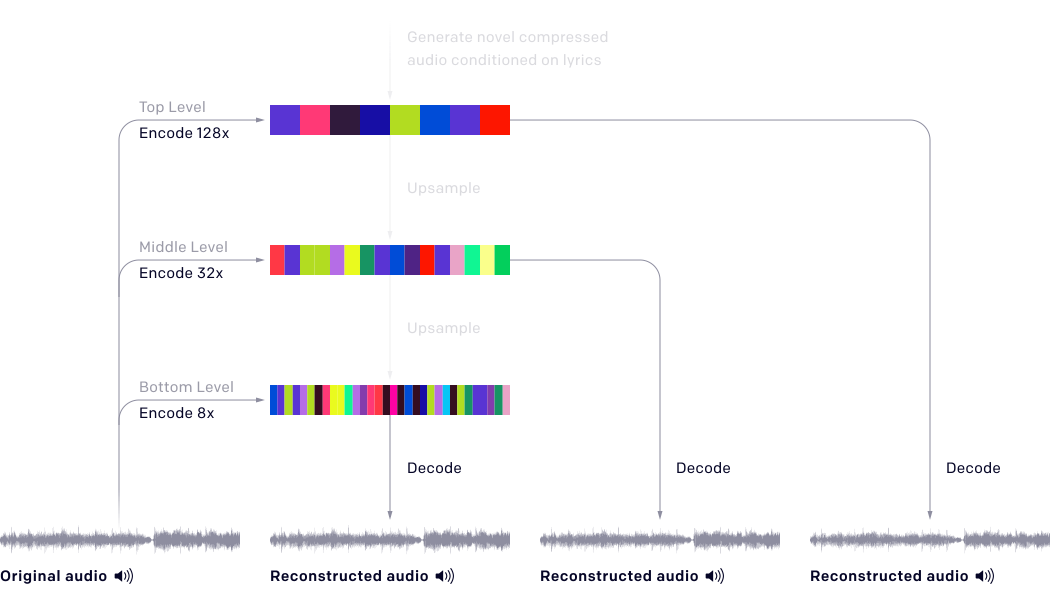
\includegraphics[width=0.8\textwidth]{literature_review/vq-vae.png}
    \caption{VQ-VAE Encoding and Compression: Successive levels further compress the raw audio data, discarding irrelevant information}
    \label{fig:jukebox_example}
\end{figure}

\subsection{Jukebox Evaluation}

Although local musical coherence, timbre among other things is good, longer term musical structure is not fully present. The upsampling process also introduces significant noise into the final audio which sounds jarring to the listener.

Another big disadvantage is the lack of parallel sampling and autoregressive nature of the model meaning that it takes multiple hours to produce one minute of music. This limits its broad applicability as its prohibitively expensive.

The model also functions much like a black box, preventing us from gaining any important information into how it is synthesising its audio. This further limits its potential uses as we cannot independently modify model parameters such as pitch and timbre of generated music.

Finally waveform based models require significant amounts of training data in order to accurately train the model and extract relevant musical features.

